% GENERATED by docs/tools/build-latex.js from docs/REPORT.md. Do not edit: change the Markdown and rebuild.
\chapter{Project Description and Design}\label{ch:design}

\section{Project planning}

\subsection{Approach and workflow}

The system was built in vertical slices, each ending in something testable, rather than layer by layer:

\begin{enumerate}
\item \textbf{Desktop shell and capture} (global shortcut, transparent overlay, frozen screenshot).
\item \textbf{Annotation tools and cropping} (shapes, masking, blur; crops at physical resolution under any display scaling).
\item \textbf{Local processing} (OCR, thumbnails, a \textquotedbl{}what will be sent\textquotedbl{} notice).
\item \textbf{AI integration} (provider abstraction, streaming, follow-ups).
\item \textbf{Cloud backend} (authentication, quotas, validation, provider routing, SSE).
\item \textbf{Cloud deployment and verification} (Firebase, Render or Cloud Run, verification script).
\item \textbf{Hardening and performance} (security review, dependency audit, latency and memory work).
\item \textbf{Documentation and evaluation} (architecture, security and deployment documents, this report).
\end{enumerate}

\subsection{Work breakdown and deliverables}

{\small
\begin{longtable}{>{\raggedright\arraybackslash}p{\dimexpr(\linewidth-8\tabcolsep)*0.069\relax}>{\raggedright\arraybackslash}p{\dimexpr(\linewidth-8\tabcolsep)*0.345\relax}>{\raggedright\arraybackslash}p{\dimexpr(\linewidth-8\tabcolsep)*0.391\relax}>{\raggedright\arraybackslash}p{\dimexpr(\linewidth-8\tabcolsep)*0.195\relax}}
\caption{Work breakdown and deliverables}\\
\toprule
\rowcolor{tblhead}\textbf{Phase} & \textbf{Work} & \textbf{Deliverable} & \textbf{Verified by} \\
\midrule
\endfirsthead
\toprule
\rowcolor{tblhead}\textbf{Phase} & \textbf{Work} & \textbf{Deliverable} & \textbf{Verified by} \\
\midrule
\endhead
\bottomrule
\endfoot
1 & Electron shell, global shortcuts, tray & App starts in the tray; shortcut opens the overlay & Electron tests \\
2 & Drawing tools, regions, masks, blur & Overlay with all tools & Overlay test at 1.5\ensuremath{\times} scaling \\
3 & Crops, OCR, privacy notice & Panel shows thumbnails, OCR text, what is sent & UI test \\
4 & Providers, streaming, follow-ups & Streamed answers, retry, stop, follow-up & Live test with a real model \\
5 & Express API, Firebase Auth, Firestore quotas & \texttt{backend/\allowbreak{}} & 13 unit and 13 emulator tests \\
6 & Render / Cloud Run deployment, verifier & \texttt{render.\allowbreak{}yaml}, \texttt{Dockerfile}, \texttt{verify-\allowbreak{}deployment.\allowbreak{}mjs} & Verifier output (\S{}8.4) \\
7 & Security review, audit, performance & \texttt{docs/\allowbreak{}SECURITY.\allowbreak{}md}, 0 vulnerabilities, latency table & \S{}7, \S{}8 \\
8 & Documentation & README files, guides, this report & Review \\
\bottomrule
\end{longtable}
}

\subsection{Risks and mitigations}

{\small
\begin{longtable}{>{\raggedright\arraybackslash}p{\dimexpr(\linewidth-10\tabcolsep)*0.211\relax}>{\raggedright\arraybackslash}p{\dimexpr(\linewidth-10\tabcolsep)*0.047\relax}>{\raggedright\arraybackslash}p{\dimexpr(\linewidth-10\tabcolsep)*0.125\relax}>{\raggedright\arraybackslash}p{\dimexpr(\linewidth-10\tabcolsep)*0.359\relax}>{\raggedright\arraybackslash}p{\dimexpr(\linewidth-10\tabcolsep)*0.258\relax}}
\caption{Risks and mitigations}\\
\toprule
\rowcolor{tblhead}\textbf{Risk} & \textbf{Likelihood} & \textbf{Impact} & \textbf{Mitigation} & \textbf{Outcome} \\
\midrule
\endfirsthead
\toprule
\rowcolor{tblhead}\textbf{Risk} & \textbf{Likelihood} & \textbf{Impact} & \textbf{Mitigation} & \textbf{Outcome} \\
\midrule
\endhead
\bottomrule
\endfoot
Model provider is slow or overloaded & High & User-visible delay & Streaming, clear loading and error states, retry, a fast model by default, a speed test per model & Observed: 3 s to 20 s time-to-first-token depending on provider load (\S{}8.3) \\
Leaked provider key & Medium & Cost, abuse & Keys only in server secrets; none in the client; no key file on Cloud Run & No secret in the repository (checked before every commit) \\
Cost or abuse by a single user & Medium & Quota exhaustion & Auth + per-user daily quota + rate limits & Verified under a 12-request burst (\S{}8.2) \\
Capture differs across Windows display scaling & Medium & Wrong crops & Capture in physical pixels; tested at 1.5\ensuremath{\times} scaling & Test passes \\
Free-tier cold starts & High & First request is slow & Documented; health check endpoint; Cloud Run \texttt{min-\allowbreak{}instances} option & Measured by the verifier \\
Cloud account unavailable (billing) & Medium & Cannot deploy to Google Cloud & Two targets: Render (free) and Cloud Run & Both documented \\
\bottomrule
\end{longtable}
}

\subsection{Tools and technology}

Electron (desktop shell), plain JavaScript (no build step, fast start), a small C\# native helper for Windows APIs, Node.js 22 with Express, Firebase Authentication and Cloud Firestore, Google Gemini API, Render or Google Cloud Run, Docker, GitHub Actions (CI), tesseract.js (local OCR), Lucide (icons).

\section{Cloud service selection}

\subsection{Selected services and why}

{\small
\begin{longtable}{>{\raggedright\arraybackslash}p{\dimexpr(\linewidth-6\tabcolsep)*0.137\relax}>{\raggedright\arraybackslash}p{\dimexpr(\linewidth-6\tabcolsep)*0.379\relax}>{\raggedright\arraybackslash}p{\dimexpr(\linewidth-6\tabcolsep)*0.484\relax}}
\caption{Selected services and why}\\
\toprule
\rowcolor{tblhead}\textbf{Need} & \textbf{Service} & \textbf{Why this one} \\
\midrule
\endfirsthead
\toprule
\rowcolor{tblhead}\textbf{Need} & \textbf{Service} & \textbf{Why this one} \\
\midrule
\endhead
\bottomrule
\endfoot
User identity & \textbf{Firebase Authentication} & Managed sign-in and short-lived signed ID tokens (JWT, one hour) that the API verifies with Google's public keys. No password database to build or protect. Supports revocation and disabling users. \\
Per-user usage and quotas & \textbf{Cloud Firestore} & A serverless document database with \textbf{transactions}, so \textquotedbl{}check the quota and add one\textquotedbl{} is atomic and concurrent requests cannot exceed the limit. Scales without servers to manage. Only counters are stored. \\
Running the API & \textbf{Render web service} (free) or \textbf{Google Cloud Run} & Managed HTTPS and certificates, deploy from Git or a container, secret environment variables, health checks. Cloud Run additionally scales instances automatically, supports least-privilege service accounts, and removes the need for any key file. \\
AI inference & \textbf{Google Gemini API} (optional: any OpenAI-compatible service) & Vision input, token streaming and web grounding in one API. Called only from the backend, so the key never reaches users. \\
Secrets & Host secret environment variables; \textbf{Secret Manager} on Cloud Run & The only place a key exists. \\
Observability & Platform logs and structured JSON logs & One line per request with request id, user id, model, outcome and latencies. No content. \\
\bottomrule
\end{longtable}
}

\subsection{Alternatives considered}

{\small
\begin{longtable}{>{\raggedright\arraybackslash}p{\dimexpr(\linewidth-6\tabcolsep)*0.111\relax}>{\raggedright\arraybackslash}p{\dimexpr(\linewidth-6\tabcolsep)*0.321\relax}>{\raggedright\arraybackslash}p{\dimexpr(\linewidth-6\tabcolsep)*0.568\relax}}
\caption{Alternatives considered}\\
\toprule
\rowcolor{tblhead}\textbf{Decision} & \textbf{Alternative} & \textbf{Why not chosen} \\
\midrule
\endfirsthead
\toprule
\rowcolor{tblhead}\textbf{Decision} & \textbf{Alternative} & \textbf{Why not chosen} \\
\midrule
\endhead
\bottomrule
\endfoot
Identity & Build our own login (database + password hashing + session tokens) & More code and more attack surface for no benefit; easy to get wrong \\
Identity & AWS Cognito / Azure AD B2C & Comparable, but Firebase integrates directly with Firestore rules and Google tooling, and has a free tier suited to a student project \\
Quota store & A relational database & A heavier service to run for a handful of counters; Firestore transactions give exactly the atomicity needed \\
Quota store & In-memory counters & Lost on restart and not shared between instances (kept only as a local-development fallback) \\
Conversation storage & Store chats in Firestore & Rejected on privacy grounds: it would mean storing screenshots and prompts. The client keeps conversations in memory only \\
Compute & Virtual machine & More to patch and secure, no automatic scaling or managed TLS \\
Compute & Cloud Functions & Long-lived streaming responses fit a container service better \\
AI & Calling the model from the desktop app & Would put the provider key in the client \\
\bottomrule
\end{longtable}
}

We did not add services for their own sake: there is no message queue, cache or extra database because no requirement needs one.

\subsection{Cost awareness}

All chosen services have free tiers sufficient for development and a demonstration (check the current limits on the providers' pricing pages before relying on them). Cost is also \emph{bounded by design}: the daily quota caps requests per user, request size is limited, upstream calls time out, and Cloud Run offers \texttt{-\allowbreak{}-\allowbreak{}max-\allowbreak{}instances} as a hard ceiling.

\section{Architecture}

\begin{figure}[htbp]
\centering
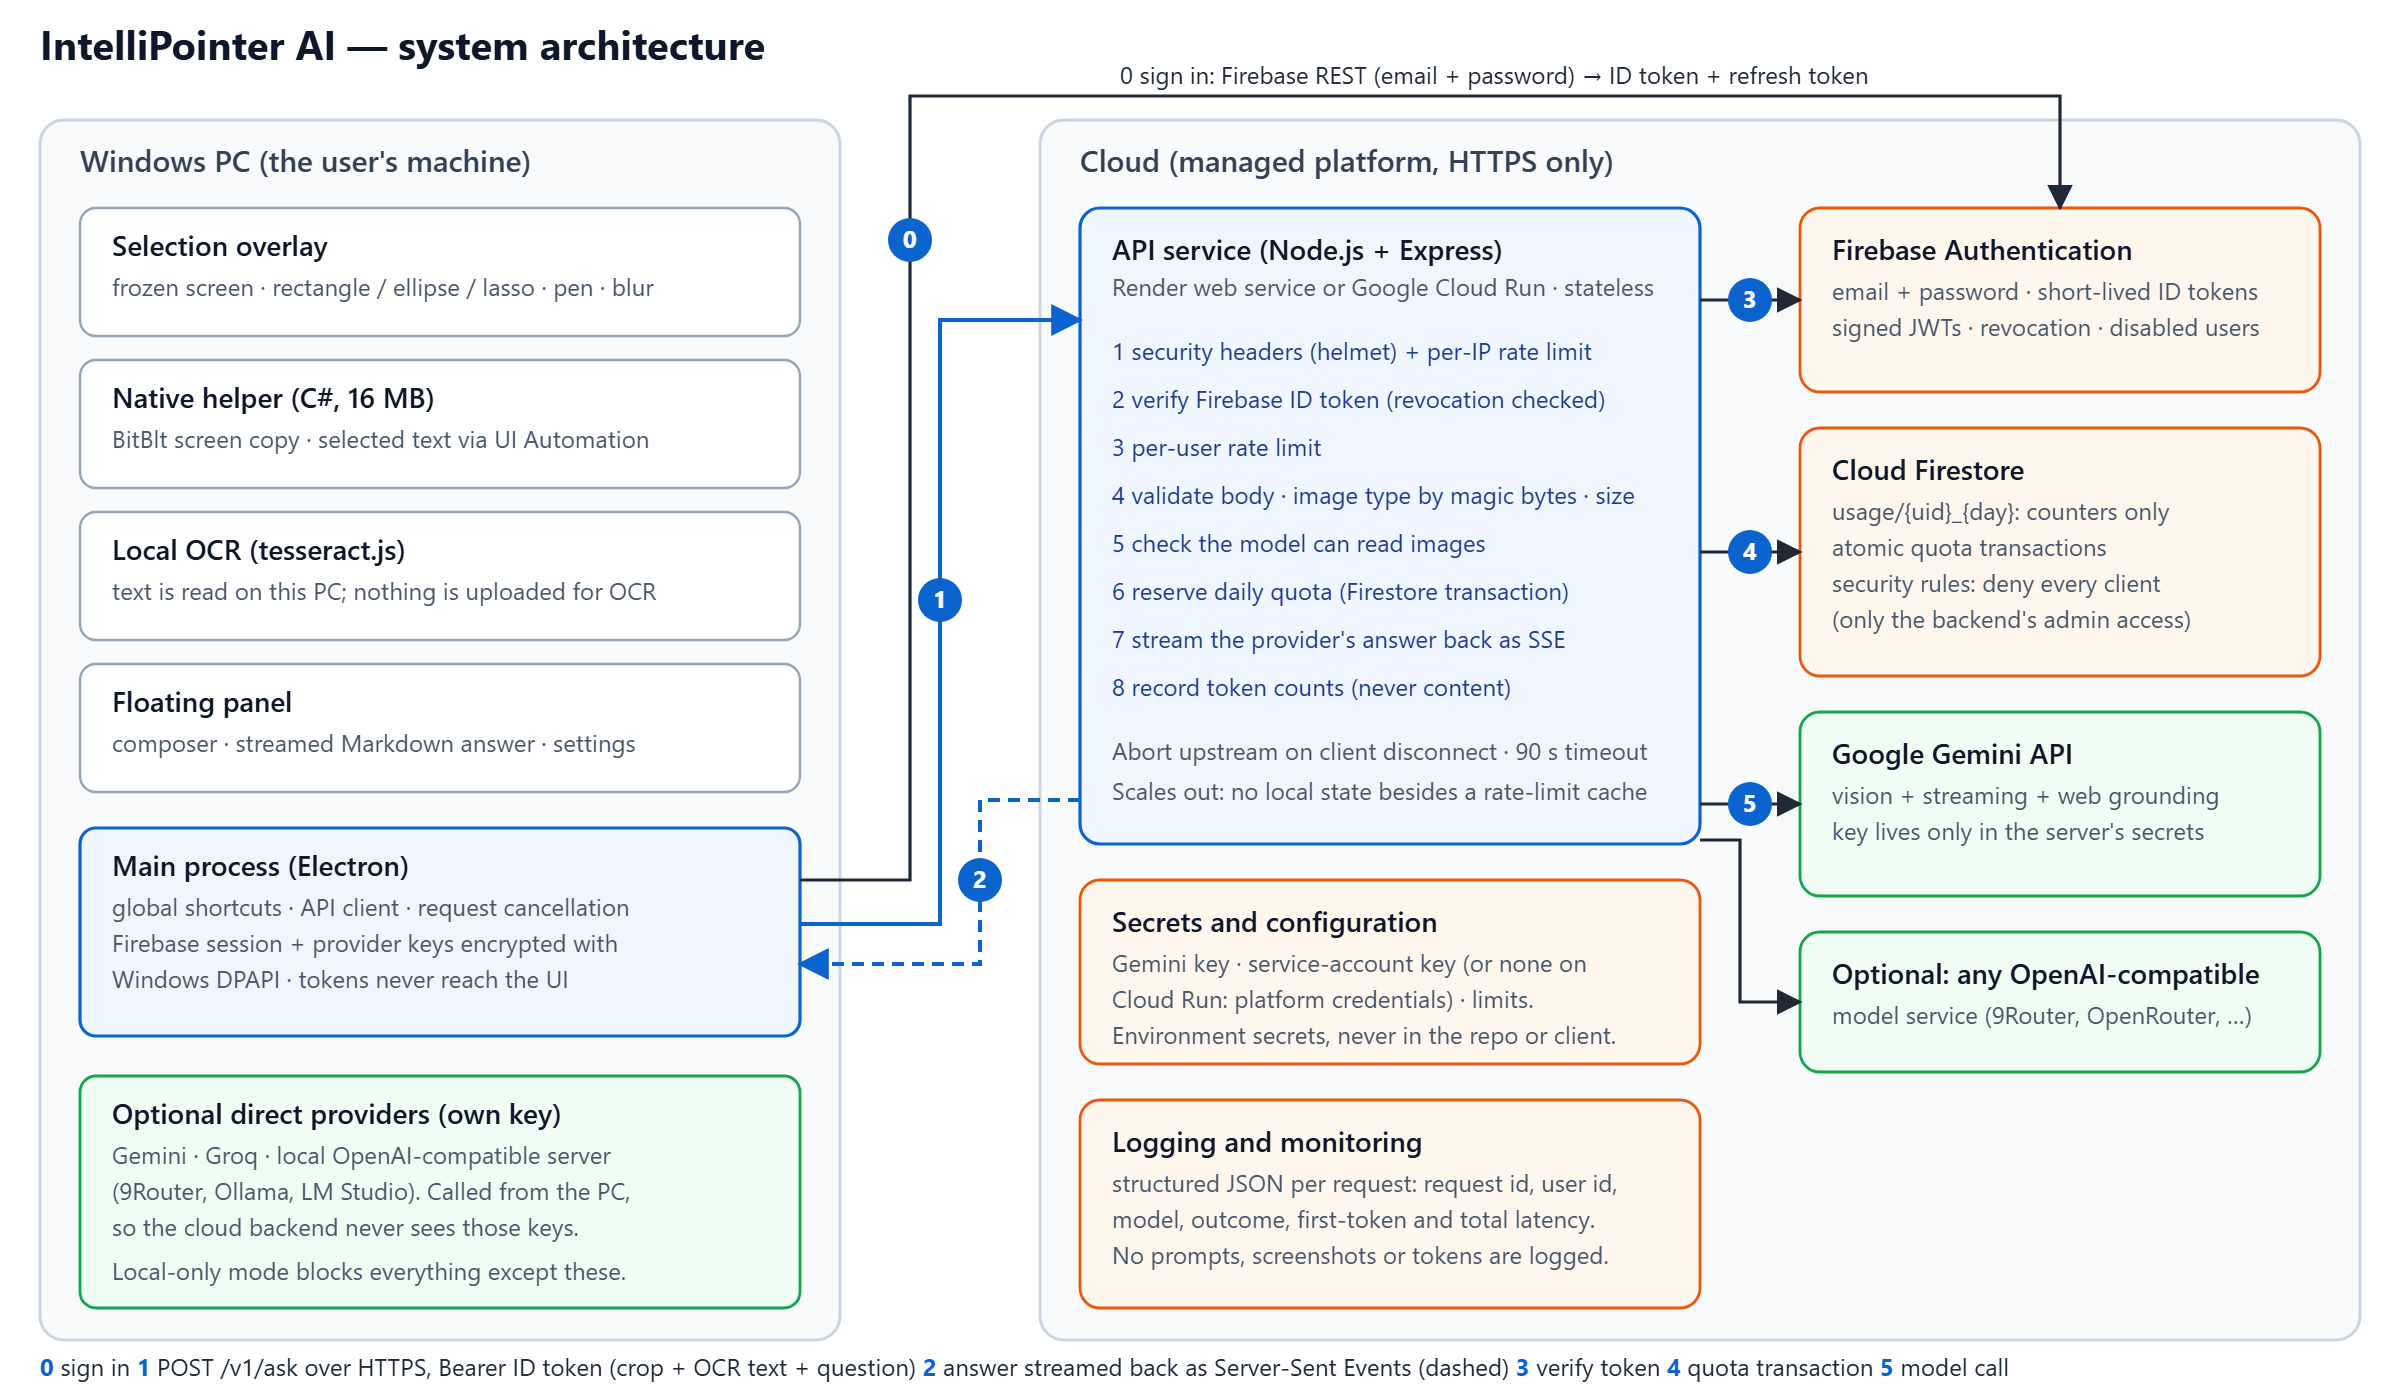
\includegraphics[width=\linewidth]{architecture.png}
\caption{System architecture. Numbered flows: 0 sign in, 1 request, 2 streamed response, 3 token verification, 4 quota transaction, 5 model call.}
\end{figure}

\subsection{Components}

\textbf{Windows client (Electron).}

\begin{itemize}
\item The \emph{main process} owns the shortcuts, the API client, request cancellation, and the encrypted Firebase session and provider keys (Windows DPAPI).
\item \emph{Overlay windows} (one per display) draw the selection tools over a frozen screenshot.
\item The \emph{panel} shows the conversation, the model menu and settings.
\item A 16 MB \emph{native helper} provides fast screen copies and reads selected text.
\item \emph{Local OCR} runs on the PC.
\item Renderers are sandboxed and see no tokens or keys.
\end{itemize}

\textbf{API service (Node.js + Express), stateless.} Per request: security headers and a per-IP rate limit \ensuremath{\rightarrow} verify the Firebase ID token (with revocation check) \ensuremath{\rightarrow} per-user rate limit \ensuremath{\rightarrow} validate the body and images (file signature, size, count) \ensuremath{\rightarrow} check the model can read images \ensuremath{\rightarrow} reserve the daily quota in a Firestore transaction \ensuremath{\rightarrow} stream the provider's answer as Server-Sent Events \ensuremath{\rightarrow} record token counts \ensuremath{\rightarrow} log the outcome.

\textbf{Firebase Authentication.} Issues and verifies identity tokens.

\textbf{Cloud Firestore.} One small document per user per day, \texttt{usage/\allowbreak{}\{uid\}\_\allowbreak{}\{YYYY-\allowbreak{}MM-\allowbreak{}DD\}}, holding only counters. Security rules deny every client; only the backend's admin access reads or writes.

\textbf{AI provider.} Gemini through its official streaming API, behind a provider registry that also accepts any OpenAI-compatible endpoint.

\subsection{One question, end to end}

\begin{figure}[htbp]
\centering
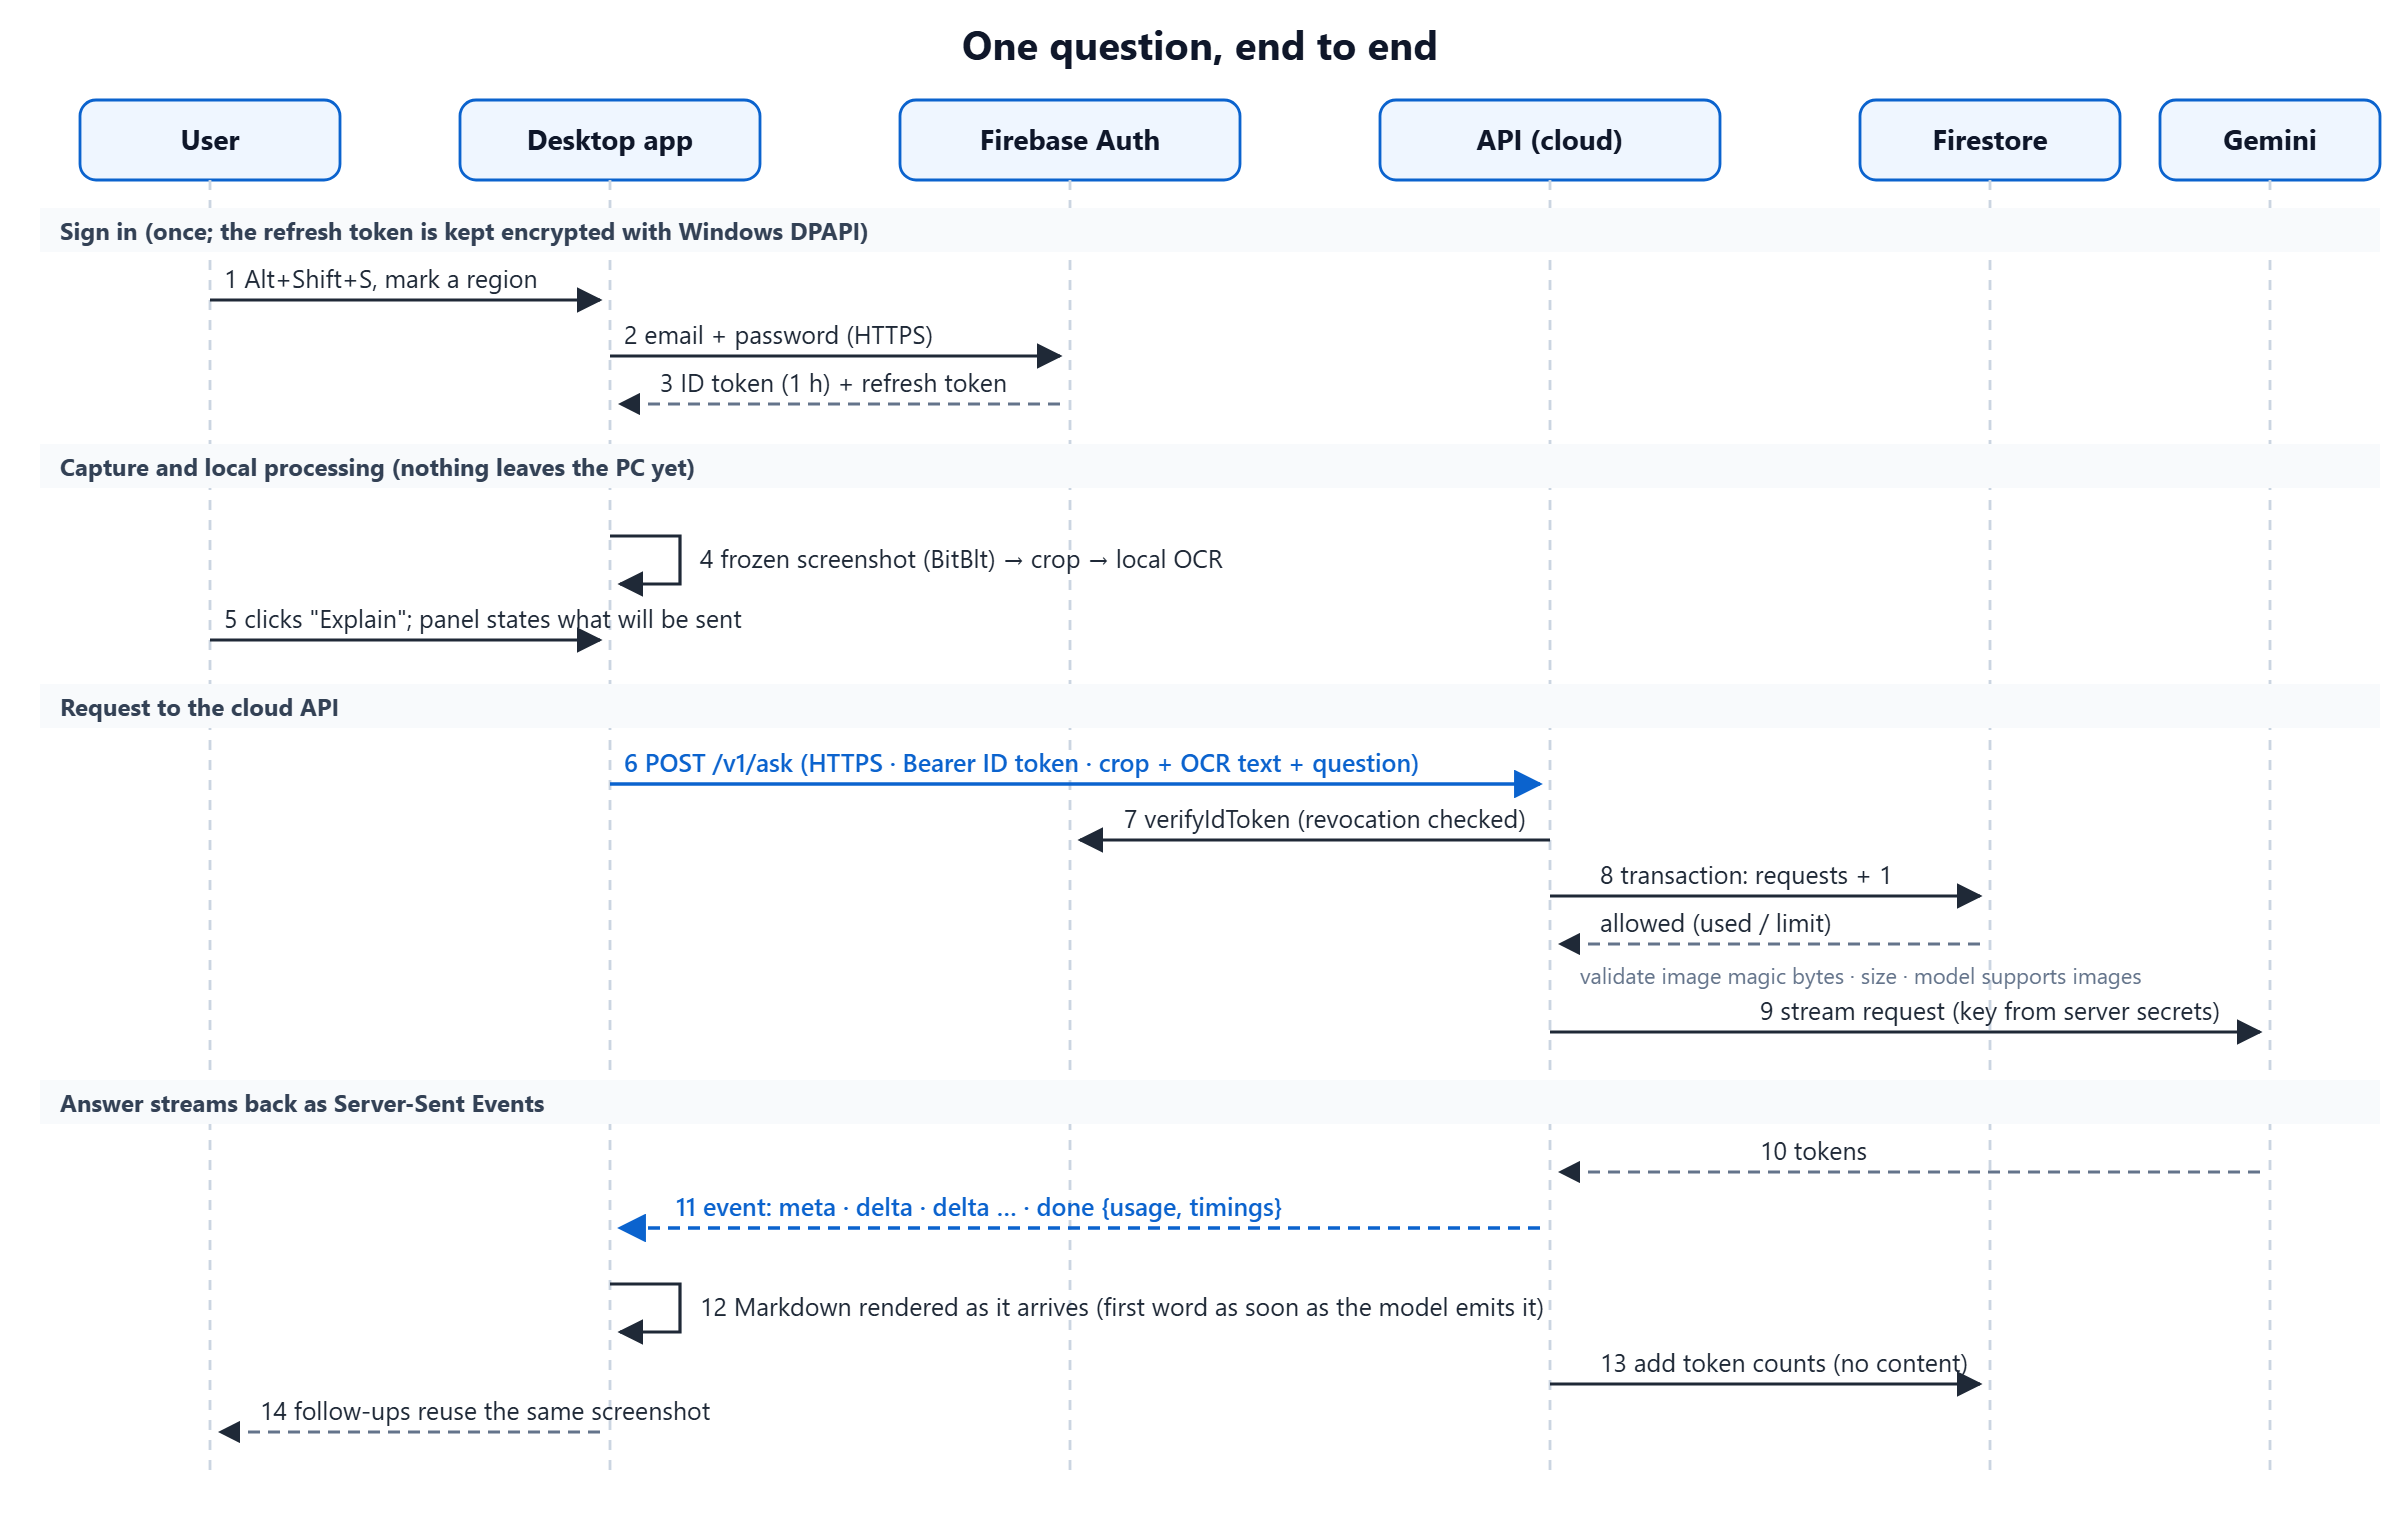
\includegraphics[width=\linewidth]{sequence.png}
\caption{Sequence of one question: sign in, local capture and OCR, authenticated request, quota transaction, streamed answer.}
\end{figure}

\subsection{Data model}

{\small
\begin{longtable}{>{\raggedright\arraybackslash}p{\dimexpr(\linewidth-6\tabcolsep)*0.161\relax}>{\raggedright\arraybackslash}p{\dimexpr(\linewidth-6\tabcolsep)*0.529\relax}>{\raggedright\arraybackslash}p{\dimexpr(\linewidth-6\tabcolsep)*0.310\relax}}
\caption{Data model}\\
\toprule
\rowcolor{tblhead}\textbf{Store} & \textbf{Content} & \textbf{Retention} \\
\midrule
\endfirsthead
\toprule
\rowcolor{tblhead}\textbf{Store} & \textbf{Content} & \textbf{Retention} \\
\midrule
\endhead
\bottomrule
\endfoot
Firestore \texttt{usage/\allowbreak{}\{uid\}\_\allowbreak{}\{day\}} & \texttt{uid}, \texttt{day}, \texttt{requests}, \texttt{inputTokens}, \texttt{outputTokens}, \texttt{lastProvider}, \texttt{lastModel}, \texttt{updatedAt} & Per day; no content \\
Desktop \texttt{\%APPDATA\%} & Non-secret settings; DPAPI-encrypted session and provider keys; a timings-only CSV and diagnostics log & Until the user clears it \\
Anywhere & Screenshots, OCR text, prompts, answers & \textbf{Never stored}; in memory until the conversation is cleared \\
\bottomrule
\end{longtable}
}

\subsection{Scalability and availability}

\begin{itemize}
\item \textbf{Horizontal scaling.} The API keeps no session state (identity is in the token, quota in Firestore), so any number of instances can serve any request. Cloud Run adds instances automatically with load.
\item \textbf{Atomic shared state.} The quota is a Firestore transaction on one small document per user-day, so instances never disagree. A single document sustains roughly one write per second, which is far above one user's request rate.
\item \textbf{Streaming.} Responses are Server-Sent Events, so the user sees text as soon as the model produces it; the server aborts the upstream call if the client leaves.
\item \textbf{Failure handling.} Upstream errors become a retryable SSE error event; the client can retry or switch model; health checks let the platform restart a failing instance; a 90-second upstream timeout prevents hung requests.
\item \textbf{Known scaling limit.} The per-minute rate limiter is per instance (in memory). The daily quota, which bounds cost, is global. A shared limiter is the next step for large deployments (\S{}9).
\end{itemize}
